\documentclass[tikz,border=12pt]{standalone}
\usepackage{amsmath,amssymb}
\usetikzlibrary{calc,arrows.meta}

\begin{document}
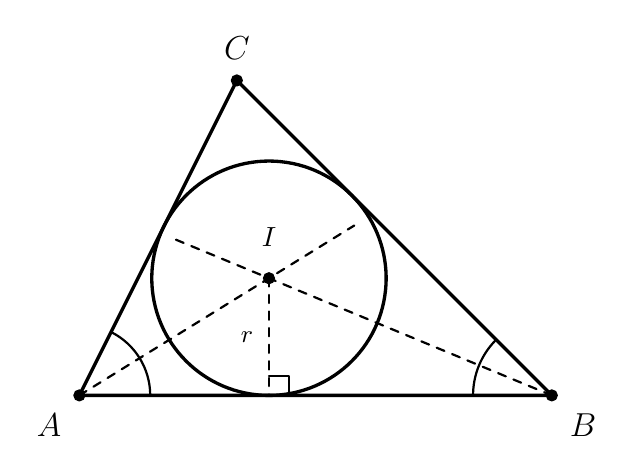
\begin{tikzpicture}[>=latex, line cap=round, line join=round]
  % Vertices of triangle ABC
  \coordinate (A) at (0, 0);
  \coordinate (B) at (6, 0);
  \coordinate (C) at (2, 4);

  % Calculated incenter and inradius:
  \coordinate (I) at (2.408, 1.488);
  \def\rIn{1.488}

  % Triangle ABC
  \draw[very thick] (A) -- (B) -- (C) -- cycle;

  % Vertices
  \filldraw[black] (A) circle (2pt) node[below left=3pt, font=\large\bfseries] {$A$};
  \filldraw[black] (B) circle (2pt) node[below right=3pt, font=\large\bfseries] {$B$};
  \filldraw[black] (C) circle (2pt) node[above=4pt, font=\large\bfseries] {$C$};

  % Inscribed circle
  \draw[very thick] (I) circle (\rIn);
  \filldraw[black] (I) circle (2pt);
  \node[above=8pt, font=\normalsize\bfseries] at (I) {$I$};

  % Dashed angle bisector lines through incenter I
  \draw[thick, dashed] (A) -- ($(A)!1.45!(I)$);
  \draw[thick] (0.9, 0) arc (0:63.4:0.9);

  \draw[thick, dashed] (B) -- ($(B)!1.35!(I)$);
  \draw[thick] ($(B) + (180:1.0)$) arc (180:135:1.0);

  % Inradius drop to base AB
  \coordinate (D) at (2.408, 0);
  \draw[thick, dashed] (I) -- (D) node[midway, left=2pt, font=\small] {$r$};
  \draw[thick] (2.408, 0.25) -- (2.658, 0.25) -- (2.658, 0); % Right angle symbol

\end{tikzpicture}
\end{document}
